% EF5342 Week 1 — Overview of the Financial System
% Pilot Beamer conversion from week1_Overview.pptx (65 source slides -> 39 frames).
% Compile: pdflatex week1_Overview.tex
% Each frame carries a [src: ...] comment mapping back to source slides
% (the content-coverage checklist; S = section divider slide in the pptx).
\documentclass[aspectratio=169]{beamer}
\usepackage{../ef5342}

\title{EF5342 Financial Systems, Markets and Instruments}
\subtitle{Week 1 --- Overview of the Financial System}
\author{Prof.\ Weikai Li}
\institute{City University of Hong Kong}
\date{Semester B 2026--2027}

\begin{document}

% ============ ADMIN ============

% [src: 1]
\begin{frame}
\titlepage
\end{frame}

% [src: 2]
\begin{frame}{About Me}
\begin{itemize}
  \item Ph.D.\ in Finance, HKUST; CFA charterholder since 2021
  \item Associate Professor of Finance; prior to joining CityU, taught at Singapore Management University
  \item Research in behavioral finance, asset pricing, and ESG, published in top journals
  \item Consultant to quant funds (Magnum Research Global, Heritage Capital Management)
  \item LinkedIn: \href{https://www.linkedin.com/in/weikai-li-ph-d-cfa-9aa65231/}{weikai-li-ph-d-cfa}
  \quad Website: \href{https://sites.google.com/view/frankweikaili/home}{sites.google.com/view/frankweikaili}
  \item Course materials (slides, LaTeX source): \href{https://github.com/franklee16/Financial-Systems-Markets-and-Instruments}{github.com/franklee16/Financial-Systems-Markets-and-Instruments}
\end{itemize}
\end{frame}

% [src: 3, 5]
\begin{frame}{Course Logistics and Assessment}
\begin{columns}
\begin{column}{0.48\textwidth}
\textbf{Logistics}
\begin{itemize}
  \item Check Canvas regularly for announcements and downloads
  \item One TA per section --- contact your section's TA for all course matters
\end{itemize}
\end{column}
\begin{column}{0.48\textwidth}
\textbf{Assessment}
\begin{itemize}
  \item 20\% individual assignments (two sets, work independently)
  \item 30\% group project
  \item 50\% final exam (MCQs + calculations, similar to assignments)
\end{itemize}
\end{column}
\end{columns}
\vspace{0.8em}
\textbf{Final exam:} one two-sided A4 cheat sheet (name on top) allowed; calculator permitted per university regulations.
\end{frame}

% [src: 4]
\begin{frame}{Group Project (30\%)}
\begin{itemize}
  \item Analyze financial market instruments or institutions; requires collecting and analyzing financial data
  \item Two topics announced in Week 2 --- your group picks one
  \item Form groups by Week 3 (max 7 students; TA re-shuffles if needed; email TA your group composition)
  \item Report (20\%) due Week 10, Sunday --- email to me
  \item Presentation (10\%): 15 minutes + 5 minutes Q\&A; all members present; Q\&A not dominated by one member
\end{itemize}
\end{frame}

% [src: 6]
\begin{frame}{My Teaching Style}
\begin{itemize}
  \item \textbf{Broad and practical}: real-world examples; figures illustrating trends and patterns; a recent case or news item opening every class
  \item \textbf{Goal}: understand \emph{why} financial markets behave as they do, and how to interpret financial news
  \item \textbf{Research-oriented}: as a research-track professor, I bring relevant academic research into class; the project teaches you to put every claim to the test with data
\end{itemize}
\note{Academic papers = future knowledge. Textbooks = 30-year-old knowledge.}
\end{frame}

% ============ PART I: FUNCTION OF FINANCIAL MARKETS ============

% [src: 7]
\section{Overview of the Financial System}

% [src: 8, 9]
\begin{frame}{Preview: The Robot-Startup Story}
\textbf{Setup:} You want to start a business manufacturing a household cleaning robot, but you have no funds. At the same time, Walter has money he wishes to invest for retirement.
\vspace{0.6em}

\textbf{Question:} If the two of you could get together, both needs could be met. \emph{How does that happen?}
\vspace{0.6em}

As simple as this example is, it highlights the importance of financial markets and financial intermediaries in our economy --- we need to understand their structure and operations before we can appreciate their role.
\end{frame}

% [src: 10]
\begin{frame}{Roadmap for Today}
We examine the role of the financial system in an advanced economy: the effects of financial markets and institutions on the economy, their structure and operations.
\vspace{0.5em}
\begin{itemize}
  \item Function of financial markets
  \item Structure of financial markets
  \item Internationalization of financial markets
  \item Function of financial intermediaries: indirect finance
  \item Types of financial intermediaries
  \item Regulation of the financial system
\end{itemize}
\end{frame}

% [src: 11, 15, 16]
\begin{frame}{Function of Financial Markets}
Channels funds from those \textbf{without} investment opportunities (``lender-savers'') to those \textbf{with} them (``borrower-spenders'') --- improving economic efficiency.
\vspace{0.6em}

\textbf{Why it matters:} save \$1,000 with no financial markets and you earn no return --- might as well put the money under your pillow. But a carpenter who can buy a new saw with that money (raising her productivity) will pay you interest for it.
\vspace{0.6em}

Financial markets produce an \textbf{efficient allocation of capital} and let consumers \textbf{time their purchases} better.
\end{frame}

% [src: 12]
\begin{frame}{Who Are the Lender-Savers and Borrower-Spenders?}
\begin{columns}
\begin{column}{0.48\textwidth}
\textbf{Lender-Savers} (surplus units)
\begin{itemize}
  \item Households
  \item Firms
  \item Government
  \item Foreigners
\end{itemize}
\end{column}
\begin{column}{0.48\textwidth}
\textbf{Borrower-Spenders} (deficit units)
\begin{itemize}
  \item Firms
  \item Government
  \item Households
  \item Foreigners
\end{itemize}
\end{column}
\end{columns}
\vspace{0.6em}
The same four sectors appear on both sides --- who is which depends on circumstances, not identity.
\end{frame}

% [src: 13]
\begin{frame}{Two Segments: Direct vs.\ Indirect Finance}
\begin{description}
  \item[Direct finance] Borrowers borrow \emph{directly} from lenders in financial markets by selling securities --- claims on the borrower's future income or assets
  \item[Indirect finance] Borrowers borrow \emph{indirectly} via financial intermediaries, which source both loanable funds and loan opportunities
\end{description}
\vspace{0.4em}
Next: the map of how funds actually flow through the system.
\end{frame}

% [src: 14]
\begin{frame}{Flows of Funds Through the Financial System}
\begin{figure}
\centering
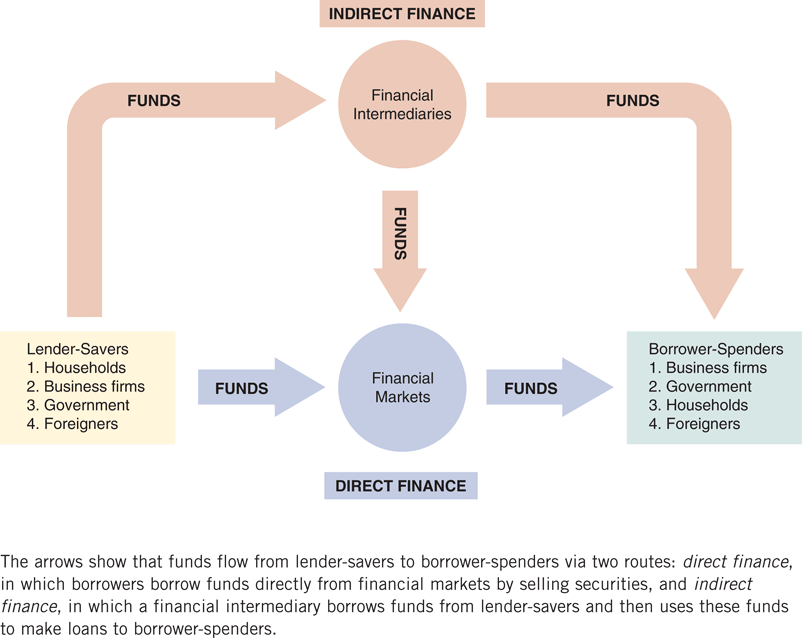
\includegraphics[height=0.70\textheight,keepaspectratio]{figures/slide02_img.png}
\caption{Mishkin, Figure 2.1}
\end{figure}
\end{frame}

% ============ PART II: STRUCTURE OF FINANCIAL MARKETS ============

% [src: 17]
\begin{frame}{Structure: Debt vs.\ Equity Markets}
Markets can be classified along several (not mutually exclusive) dimensions.
\begin{columns}
\begin{column}{0.48\textwidth}
\textbf{Debt markets}
\begin{itemize}
  \item Money market: maturity $< 1$ year
  \item Intermediate term: in between
  \item Long term: maturity $> 10$ years
  \item Global total $\approx$ \$353 trillion (Q1 2026, IIF Global Debt Monitor)
\end{itemize}
\end{column}
\begin{column}{0.48\textwidth}
\textbf{Equity markets}
\begin{itemize}
  \item Ownership claim in the firm
  \item Pays dividends --- in theory, forever
  \item Voting rights
  \item Global market cap $\approx$ \$158 trillion (end-2025, WFE/SIFMA)
\end{itemize}
\end{column}
\end{columns}
\end{frame}

% [src: 18, 19]
\begin{frame}{The Global Debt Market}
\begin{figure}
\centering
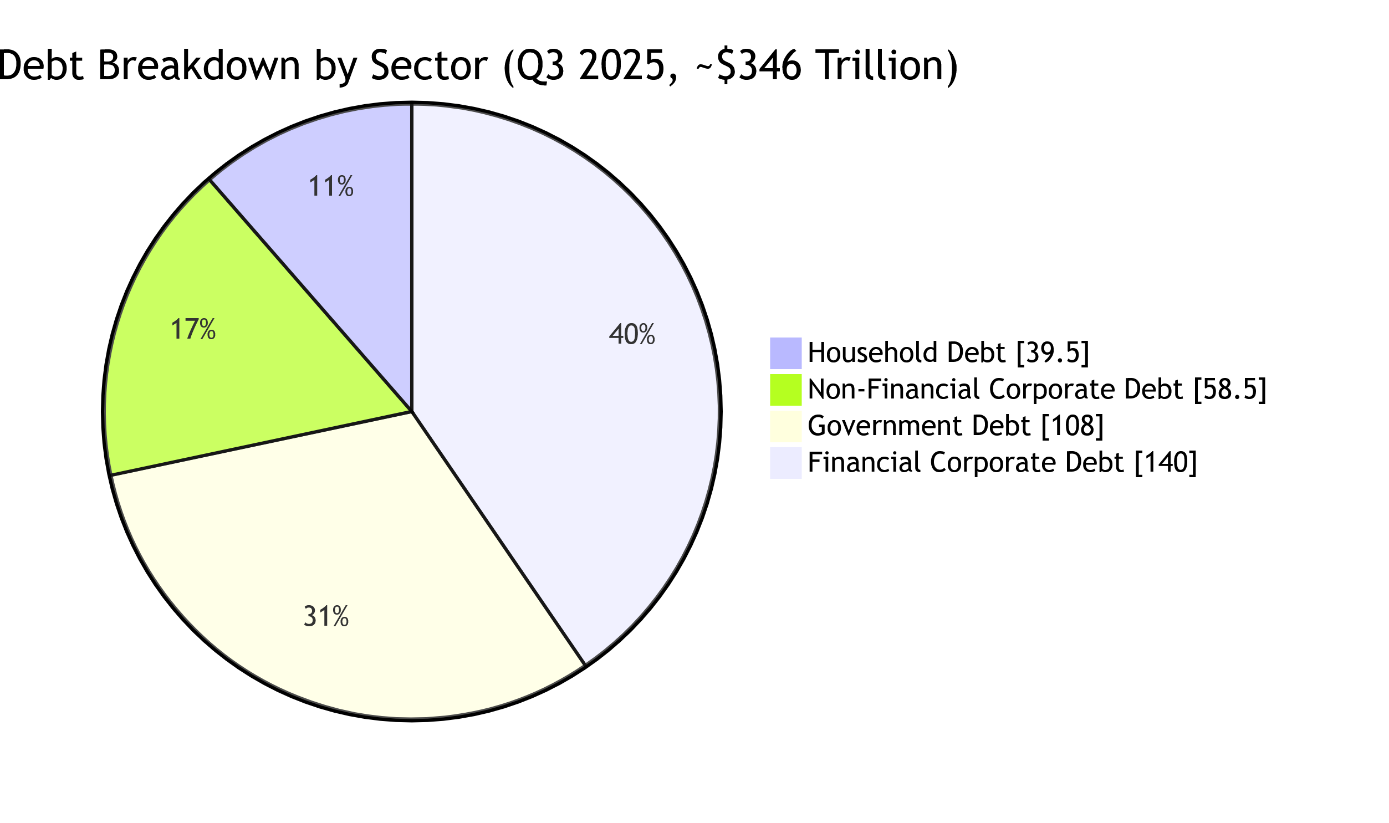
\includegraphics[width=0.62\textwidth]{figures/slide18_img_flat.png}
\end{figure}
\begin{center}
\small Source: Institute of International Finance (IIF), Global Debt Monitor (chart data as of Q3 2025)
\end{center}
\note{Breakdown categories: government debt (central/state/local); financial corporate debt (banks and other FIs); non-financial corporate debt (bonds and loans); household debt (mortgages, consumer loans).}
\end{frame}

% [src: 19]
\begin{frame}{Global Debt: Sector Composition}
\begin{figure}
\centering
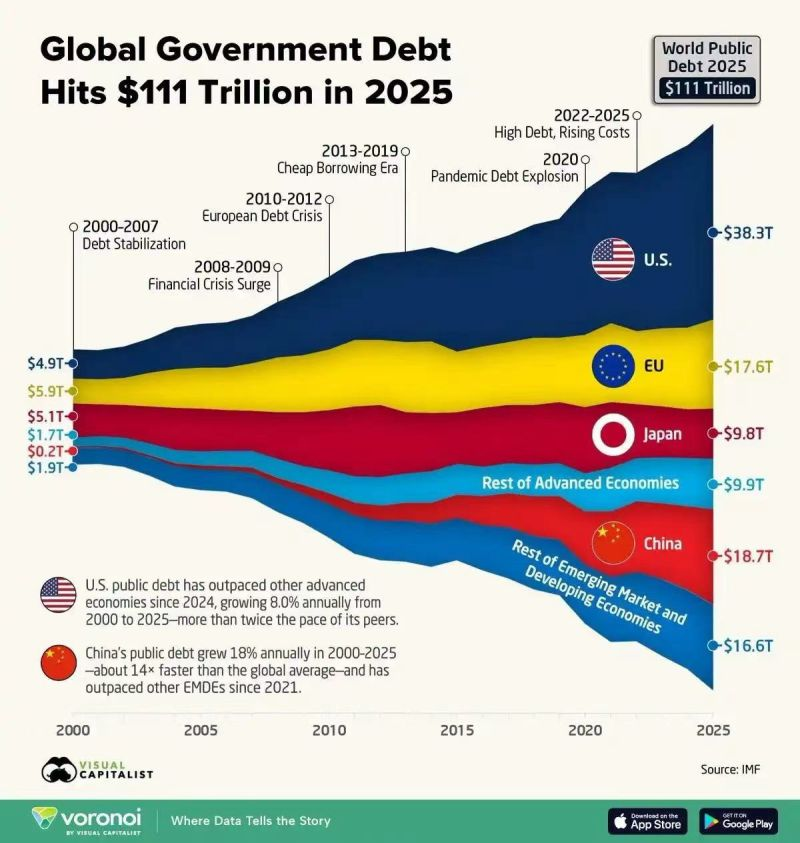
\includegraphics[height=0.68\textheight,keepaspectratio]{figures/slide19_img.jpg}
\end{figure}
\begin{center}
\small Source: Institute of International Finance (IIF), Global Debt Monitor (chart data as of 2025)
\end{center}
\end{frame}

% [src: 20]
\begin{frame}{The Global Equity Market}
\begin{figure}
\centering
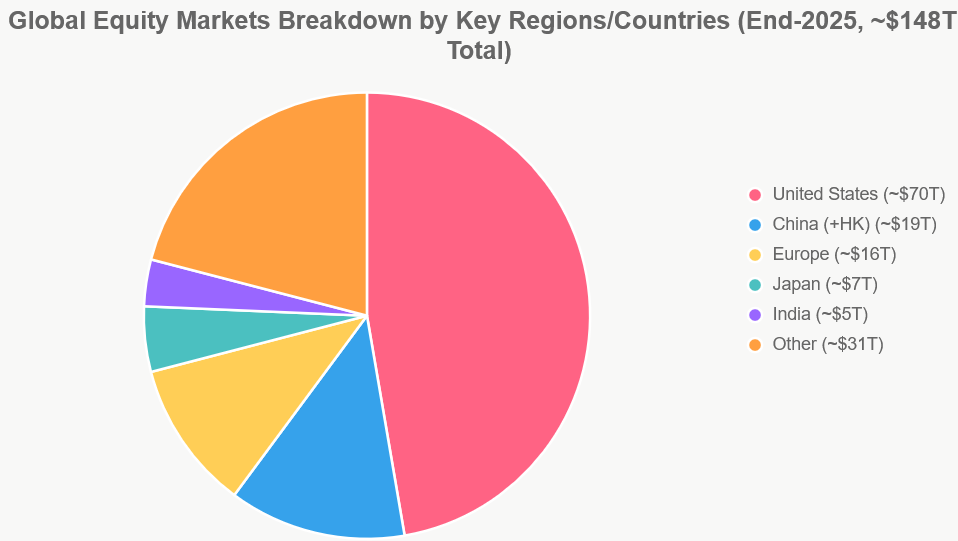
\includegraphics[height=0.80\textheight,keepaspectratio]{figures/slide20_img_flat.png}
\end{figure}
\begin{center}
\small Source: World Federation of Exchanges (WFE); chart data as of end-2025
\end{center}
\end{frame}

% [src: 21, 22]
\begin{frame}{Primary vs.\ Secondary Markets}
\begin{description}
  \item[Primary market] New security issues sold to initial buyers; typically involves an investment bank that \emph{underwrites} the offering
  \item[Secondary market] Previously issued securities bought and sold (NYSE, Nasdaq, HKEX); involves brokers and dealers
\end{description}
\vspace{0.4em}
Firms get no new capital from the secondary market, yet it serves two functions:
\begin{itemize}
  \item \textbf{Liquidity} --- easy to buy and sell the company's securities
  \item \textbf{Price discovery} --- establishes prices useful for valuing the firm
\end{itemize}
\note{Broker: buys/sells securities on behalf of clients, charges a commission. Dealer (principal / market maker): buys and sells for their own account.}
\end{frame}

% [src: 23]
\begin{frame}{Secondary Markets: Exchanges vs.\ Over-the-Counter}
\begin{description}
  \item[Exchanges] Trades conducted in central locations --- e.g., NYSE, HKEX
  \item[Over-the-counter (OTC)] Dealers at different locations buy and sell; best example is the market for U.S.\ Treasury securities
\end{description}
\note{Exchange: formal organized marketplace with strict rules, centralized matching, public price/volume disclosure. OTC: decentralized network of dealers negotiating directly.}
\end{frame}

% [src: 24]
\begin{frame}{Classifying Markets by Maturity}
\begin{description}
  \item[Money market] Short-term instruments, maturity $< 1$ year
  \item[Capital market] Long-term instruments, maturity $> 1$ year, plus equities (no finite maturity)
\end{description}
\end{frame}

% ============ PART III: INTERNATIONALIZATION ============

% [src: 25]
\begin{frame}{Internationalization: Foreign Bonds and Eurobonds}
\textbf{Foreign bond} --- issued in a domestic market by a foreign entity, denominated in the domestic currency.
\emph{Example:} a Japanese company issues a USD-denominated bond in the U.S.
\vspace{0.5em}

\textbf{Eurobond} --- issued in a currency that is not native to the country or market where it is issued.
\emph{Example:} a Japanese company issues a USD-denominated bond in London.
\begin{itemize}
  \item Over 80\% of new bonds are Eurobonds
  \item Attractive for \textbf{regulatory arbitrage}
\end{itemize}
\end{frame}

% [src: 26]
\begin{frame}{Case: ``Wonton Bonds'' in Hong Kong}
Foreign bonds denominated in HKD, issued by non-HK entities --- mainly supranational / multilateral development banks (AIIB, IFC/World Bank, ADB) and some foreign banks and corporates.
\vspace{0.4em}
\begin{itemize}
  \item Often sustainable / social / green labeled
  \item Publicly syndicated --- broader investor access than private deals
  \item Attractive in low-rate environments for diversification away from USD
  \item Help HK banks and treasuries deploy excess HKD liquidity into high-quality assets
\end{itemize}
\end{frame}

% [src: 27]
\begin{frame}{The Eurocurrency Market}
An international, largely \textbf{unregulated} network where currencies are deposited, lent, and borrowed \emph{outside their country of origin}.
\begin{itemize}
  \item \textbf{Eurodollars}: U.S.\ dollars deposited in (say) London; \textbf{Euroyen}: yen deposited in New York
  \item Chosen over domestic banks for lower borrowing rates and higher deposit rates, situationally
  \item Why? Fewer regulatory requirements, different tax laws, and typically no interest-rate caps
\end{itemize}
\end{frame}

% [src: 28]
\begin{frame}{Eurocurrency Market: Pros and Cons}
\begin{table}
\centering
\small
\begin{tabular}{p{0.46\textwidth}p{0.46\textwidth}}
\toprule
\textbf{Advantage} & \textbf{Disadvantage / Risk} \\
\midrule
Lower borrowing costs: fewer regulations allow competitive rates & Regulatory gaps: transnational nature complicates oversight \\
Higher deposit returns: banks can offer better rates & No lender of last resort: deposits lack a central-bank safety net \\
Efficient fund management: hedging currency risk, global cash management & Increased systemic risk: size and interconnectedness amplify shocks \\
Key source of trade finance: facilitates over 90\% of international trade & \\
\bottomrule
\end{tabular}
\end{table}
\end{frame}

% [src: 29]
\begin{frame}{World Stock Market Indexes}
Published daily (e.g., \href{http://www.finance.yahoo.com}{finance.yahoo.com}). The most important:
\vspace{0.3em}
\begin{columns}
\begin{column}{0.48\textwidth}
\begin{itemize}
  \item \textbf{DJIA} --- 30 largest U.S.\ public corporations
  \item \textbf{S\&P 500} --- 500 largest U.S.\ companies
  \item \textbf{Nasdaq Composite} --- all Nasdaq stocks; most U.S.\ technology names
\end{itemize}
\end{column}
\begin{column}{0.48\textwidth}
\begin{itemize}
  \item \textbf{FTSE 100} --- 100 largest UK companies (LSE)
  \item \textbf{DAX} --- 30 largest German companies (Frankfurt)
  \item \textbf{CAC 40} --- 40 largest French companies (Euronext Paris)
  \item \textbf{Hang Seng} --- largest HK-listed companies
  \item \textbf{Straits Times} --- 30 largest companies (SGX)
\end{itemize}
\end{column}
\end{columns}
\end{frame}

% ============ PART IV: FINANCIAL INTERMEDIARIES ============

% [src: 30, 31]
\begin{frame}{Indirect Finance: Financial Intermediation}
\begin{figure}
\centering
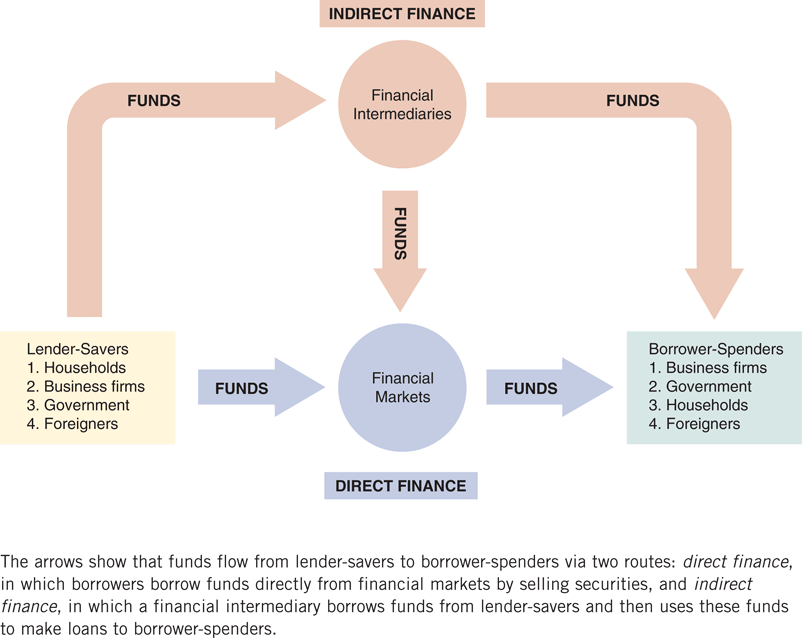
\includegraphics[height=0.58\textheight,keepaspectratio]{figures/slide03_img.png}
\end{figure}
Instead of savers lending directly to borrowers, an intermediary (such as a bank) acts as the middleman: it \textbf{obtains funds from savers}, then \textbf{makes loans and investments to borrowers}.
\end{frame}

% [src: 32]
\begin{frame}{Intermediation Dominates Direct Finance}
Financial intermediation is the \textbf{primary} means of moving funds from lenders to borrowers.
\begin{itemize}
  \item More important than direct finance in capital markets
  \item In Germany and Japan, intermediary financing exceeds capital-market financing \textbf{10-fold}
  \item Exists because direct finance suffers from: \textbf{transaction costs}, \textbf{risk sharing}, and \textbf{asymmetric information}
\end{itemize}
\end{frame}

% [src: 33, 34]
\begin{frame}{Reason 1: Transaction Costs and Liquidity Services}
FIs make profits by \textbf{reducing transaction costs}, via expertise and \textbf{economies of scale}.
\vspace{0.4em}
Low transaction costs also enable \textbf{liquidity services} --- making transactions easier for customers:
\begin{itemize}
  \item Checking accounts let depositors pay bills easily
  \item HK depositors earn interest on savings yet can convert to goods and services at any time
\end{itemize}
\end{frame}

% [src: 35]
\begin{frame}{Reason 2: Risk Sharing and Asset Transformation}
FIs reduce investors' exposure to \textbf{unsystematic risk}:
\begin{itemize}
  \item FIs create and sell low-risk assets to one party, buy higher-risk assets from another --- \textbf{asset transformation}: risky assets turned into safer assets
  \item E.g., banks lend to risky firms yet issue deposits that are almost risk-free
  \item Possible due to economies of scale: buy a range of assets, pool them, sell rights to the diversified pool
\end{itemize}
\end{frame}

% [src: 36, 37, 38, 39]
\begin{frame}{Reason 3: Asymmetric Information}
One party lacks crucial information about the other. Two fronts:
\vspace{0.3em}
\begin{description}
  \item[Adverse selection] \emph{Before} the transaction: the potential borrowers most eager to borrow are the ones most likely to produce adverse outcomes (cf.\ unhealthy people most eager to buy insurance)
  \item[Moral hazard] \emph{After} the transaction: the borrower has incentives to engage in undesirable activities that make repayment less likely (cf.\ insured people taking more risks); a conflict of interest
\end{description}
\vspace{0.3em}
FIs have expertise to mitigate both --- and profit from it. How they do it: throughout this course.
\end{frame}

% [src: 40, 41]
\begin{frame}{Economies of Scope --- and Conflicts of Interest}
\textbf{Economies of scope}: FIs lower the cost of information by reusing it across services --- bank accounts, mortgages, insurance, retirement savings.
\emph{Example:} a mortgage applicant's banker can suggest a homeowner checking account, a credit card for moving costs, and home insurance.
\vspace{0.4em}

\textbf{But} multiple services create \textbf{conflicts of interest} --- one area of the FI hiding information from another:
\begin{itemize}
  \item Selling for commissions and quotas
  \item Promoting proprietary ``in-house'' products
  \item Data-driven exploitation
\end{itemize}
This can make financial markets \emph{less} efficient and reduce consumer welfare.
\end{frame}

% [src: 42]
\begin{frame}{Types of Financial Intermediaries}
\begin{figure}
\centering
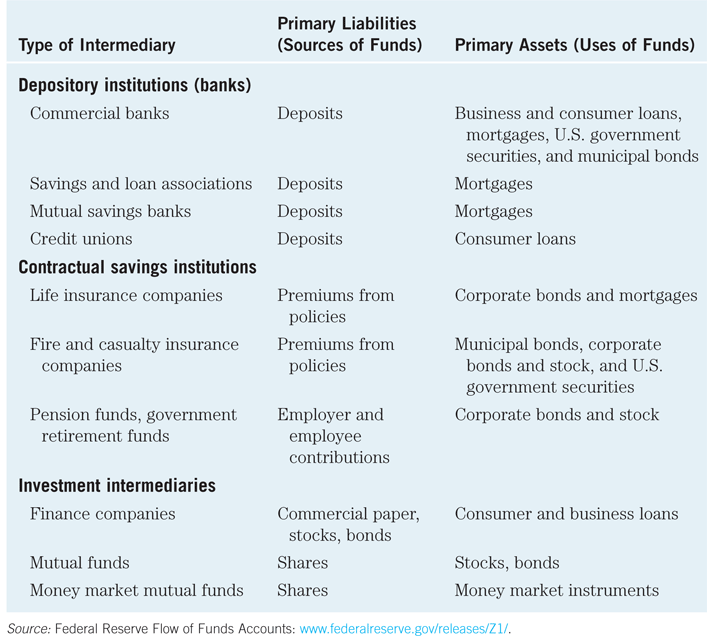
\includegraphics[height=0.70\textheight,keepaspectratio]{figures/slide04_img.png}
\caption{Mishkin, Table 2.1 --- Primary Assets and Liabilities of Financial Intermediaries}
\end{figure}
\end{frame}

% [src: 43]
\begin{frame}{Principal U.S.\ Financial Intermediaries by Asset Size}
\begin{figure}
\centering
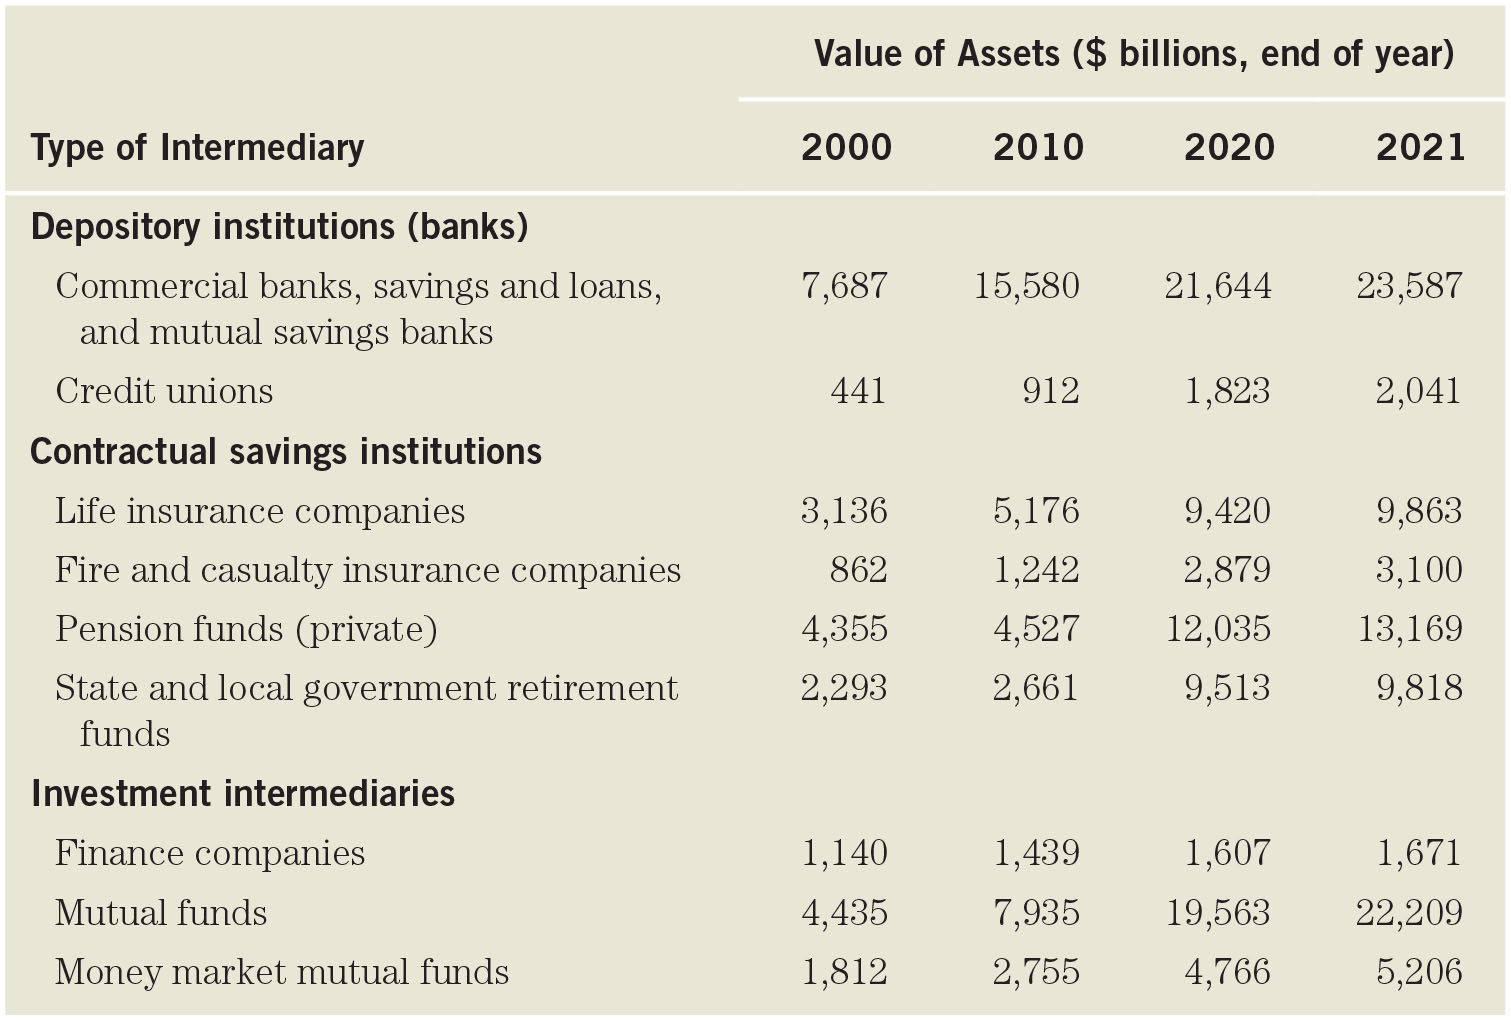
\includegraphics[height=0.80\textheight,keepaspectratio]{figures/slide05_img.jpg}
\end{figure}
\end{frame}

% [src: 44, 45]
\begin{frame}{Depository Institutions (Banks)}
Accept deposits and make loans --- commercial banks and thrifts.
\begin{description}
  \item[Commercial banks] Raise funds via current accounts, savings accounts, and time deposits; lend to commercial, consumer, and mortgage borrowers. The largest FI group, with the most diversified asset portfolios
  \item[Thrifts: S\&Ls, mutual savings banks, credit unions] Raise funds via savings, time, and checkable deposits; mostly mortgage and consumer lending. Mutual savings banks and credit unions are depositor-owned; credit union members typically share a common bond (e.g., a company's workers)
\end{description}
\note{Credit unions: member-owned, not-for-profit cooperatives providing banking-like services.}
\end{frame}

% [src: 46]
\begin{frame}{Contractual Savings Institutions}
Acquire funds at \textbf{periodic intervals on a contractual basis}; payout requirements are fairly predictable.
\begin{description}
  \item[Life insurance] Funds from premiums; can hold less liquid, longer-maturity corporate bonds and mortgages --- actuarial payouts are predictable
  \item[Fire and casualty insurance] Funds from premiums; must hold mostly liquid government and corporate securities --- losses are hard to predict
  \item[Pension and government retirement funds] Contributions from employee and employer payrolls; invest in corporate securities; pay retirement income via annuities
\end{description}
\end{frame}

% [src: 47, 48]
\begin{frame}{Other Intermediaries}
\begin{description}
  \item[Finance companies] Sell commercial paper, issue bonds and stocks; lend to consumers (durables) and small businesses
  \item[Mutual funds] Sell shares to individual investors; purchase diversified portfolios of stocks and bonds
  \item[Money market mutual funds] Sell checkable deposit-like shares; hold liquid, safe short-term money-market instruments
  \item[Hedge funds] Large minimum investments (\$\text{100,000}+), long lock-ups, few regulations; leverage and derivatives across asset classes
  \item[Investment banks] Advise on securities issuance, underwrite offerings, M\&A advisory, deal in security markets
\end{description}
\note{Finance companies: non-bank lenders specializing in consumer/business loans; do not accept deposits.}
\end{frame}

% ============ PART V: REGULATION ============

% [src: 49, 50]
\begin{frame}{U.S.\ Regulatory Agencies}
\begin{columns}
\begin{column}{0.5\textwidth}
\begin{figure}
\centering
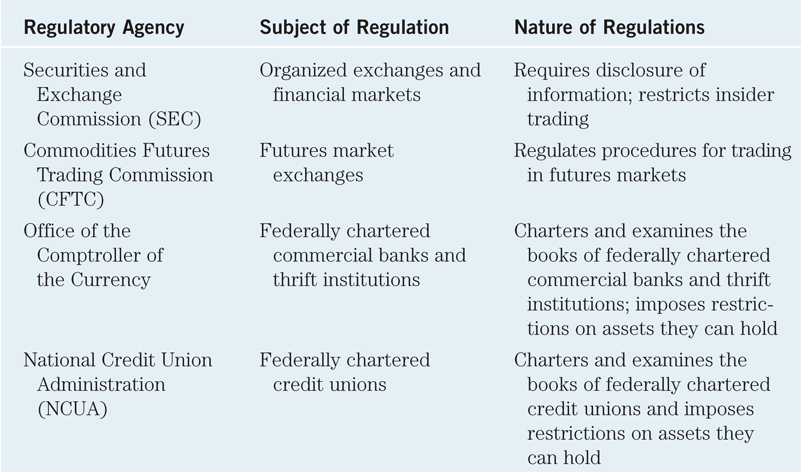
\includegraphics[width=\textwidth]{figures/slide06_img.png}
\end{figure}
\end{column}
\begin{column}{0.5\textwidth}
\begin{figure}
\centering

\includegraphics[width=\textwidth]{figures/slide07_img.png}
\end{figure}
\end{column}
\end{columns}
\begin{center}
\small Mishkin, Table 2.3 --- Principal Regulatory Agencies of the U.S.\ Financial System
\end{center}
\end{frame}

% [src: 51]
\begin{frame}{Regulatory Agencies in Hong Kong}
\begin{description}
  \item[HKMA --- Hong Kong Monetary Authority] De facto central bank: banking stability, monetary policy (Linked Exchange Rate System), prudential supervision
  \item[SFC --- Securities and Futures Commission] Market integrity, investor protection, supervision of securities and futures activities
  \item[IA --- Insurance Authority] Prudential supervision of insurers; conduct regulation of intermediaries
  \item[MPFA --- MPF Schemes Authority] Regulates and supervises the Mandatory Provident Fund system
\end{description}
\end{frame}

% [src: 52, 53, 54]
\begin{frame}{Why Regulate?}
\textbf{1. Increase investor information.} Asymmetric information causes adverse selection and moral hazard, hindering efficient market operation and driving investors away. The SEC requires disclosure of sales, assets, and earnings, and restricts trading by corporate insiders --- increasing information available to investors.
\vspace{0.4em}

\textbf{2. Ensure soundness of FIs.} Depositors cannot easily assess whether an institution is sound; doubts can trigger withdrawals from \emph{both sound and unsound} institutions --- a financial panic (bank run) with large public losses and serious economic damage.
\end{frame}

% [src: 55]
\begin{frame}{Six Types of Regulation}
To protect the public from financial panics, governments impose:
\begin{enumerate}
  \item Restrictions on entry
  \item Disclosure
  \item Restrictions on assets and activities
  \item Deposit insurance
  \item Limits on competition
  \item Restrictions on interest rates
\end{enumerate}
\vspace{0.3em}
Each in turn on the next frames.
\end{frame}

% [src: 56, 57, 58]
\begin{frame}{Regulation 1--3: Entry, Disclosure, Assets}
\textbf{Restrictions on entry} --- tight rules on who may set up an FI. In the U.S., a charter from state or federal government requires impeccable credentials and substantial initial funds. In HK, a license from the HKMA or SFC under stringent criteria.
\vspace{0.3em}

\textbf{Disclosure} --- strict reporting: bookkeeping must follow strict principles, books are periodically inspected, certain information must be made public.
\vspace{0.3em}

\textbf{Restrictions on assets and activities} --- restrict FIs from engaging in certain risky activities and from holding risky assets (or more of them than is prudent), so depositors' funds are safe.
\end{frame}

% [src: 59]
\begin{frame}{Regulation 4: Deposit Insurance}
Government insures deposits against FI failure.
\begin{center}
\begin{tabular}{lll}
\toprule
 & United States (FDIC) & Hong Kong (DPS) \\
\midrule
Coverage & USD 250{,}000 per account (since 2008) & HK\$800{,}000 per depositor per bank (since Oct 2024) \\
Applies to & Commercial and mutual savings banks & Licensed banks \\
\bottomrule
\end{tabular}
\end{center}
\end{frame}

% [src: 60, 61]
\begin{frame}{Regulation 5--6: Competition and Interest Rates}
\textbf{Limits on competition.} Evidence that competition among FIs promotes harmful failures is weak --- yet many restrictions exist. U.S.\ banks were once barred from branching across states; in HK a bank must inform the HKMA and obtain a no-objection before opening a branch.
\vspace{0.3em}

\textbf{Restrictions on interest rates.} Instituted on the belief that unrestricted deposit-rate competition encouraged Great-Depression-era bank failures; later evidence did not support this view, and the restrictions have been abolished.
\end{frame}

% [src: 62]
\begin{frame}{A Third Reason: Improve Monetary Control}
Banks play a central role in determining the money supply, which affects many aspects of the economy.
\begin{itemize}
  \item \textbf{Reserve requirements}: depository institutions must keep a fraction of deposits in accounts with the Fed
  \item This helps the Fed exercise more precise control over the money supply
\end{itemize}
\end{frame}

% [src: 63]
\begin{frame}{Financial Regulation Abroad}
Many countries with similar economic systems --- Japan, Canada, Western Europe, China, Singapore --- implement regulation consistent with the U.S.\ model:
\begin{itemize}
  \item Financial reporting for FIs is required
  \item Financial intermediaries are heavily regulated
\end{itemize}
\vspace{0.3em}
However, U.S.\ banks are said to be \emph{more} regulated than banks elsewhere along the dimensions of branching and services.
\end{frame}

% ============ SUMMARY ============

% [src: 64, 65]
\begin{frame}{Summary}
\begin{description}
  \item[Function of financial markets] Flow of funds through the system; the role of intermediaries
  \item[Structure of financial markets] By instrument type, purpose, organization, and time horizon
  \item[Internationalization] Debt and equity markets in the international setting
  \item[Function of financial intermediaries] Reducing transaction costs, facilitating risk sharing, reducing information asymmetry
  \item[Types of intermediaries] The landscape, examined further in later weeks
  \item[Regulation of the financial system] The agencies overseeing institutions and markets
\end{description}
\end{frame}

\end{document}
